\documentclass[ucs]{beamer}
\usepackage{polski}
\usepackage[utf8]{inputenc}

\usetheme{Ilmenau}

\title{Projekt i realizacja stanowiska laboratoryjnego do badania zależności czasowych w sieci EtherCAT}
\author{Damian Karbowiak}
\date{20 marzec 2013}
\begin{document}

\begin{frame}
  \titlepage
\end{frame}

\section{Wstęp}
\subsection{}
\begin{frame}
\frametitle{Opis}
Zakres pracy obejmuję projekt i realizację stanowiska laboratoryjnego złożonego z co najmniej dwóch sterowników produkcji Beckhoff do prezentacji zależności czasowych z sieci EtherCAT. Do tego celu oprócz sterowników należy użyć serwonapędów.
\end{frame}

\begin{frame}
\frametitle{Plan pracy}
\begin{enumerate}
    \item Zapoznanie się ze sterownikami Beckhoff oraz oprogramowaniem TwinCAT
    \item Zapoznanie się z dostępnymi serwonapędami Beckhoff
    \item Projekt i realizacja stanowiska
    \item Przygotowanie stanowiska do współpracy z systemem wizualizacji
    \item Testowanie i uruchamianie
\end{enumerate}
\end{frame}

\begin{frame}
\frametitle{Stanowisko typ 1}
\begin{figure}[!htb]	
\centering 	          
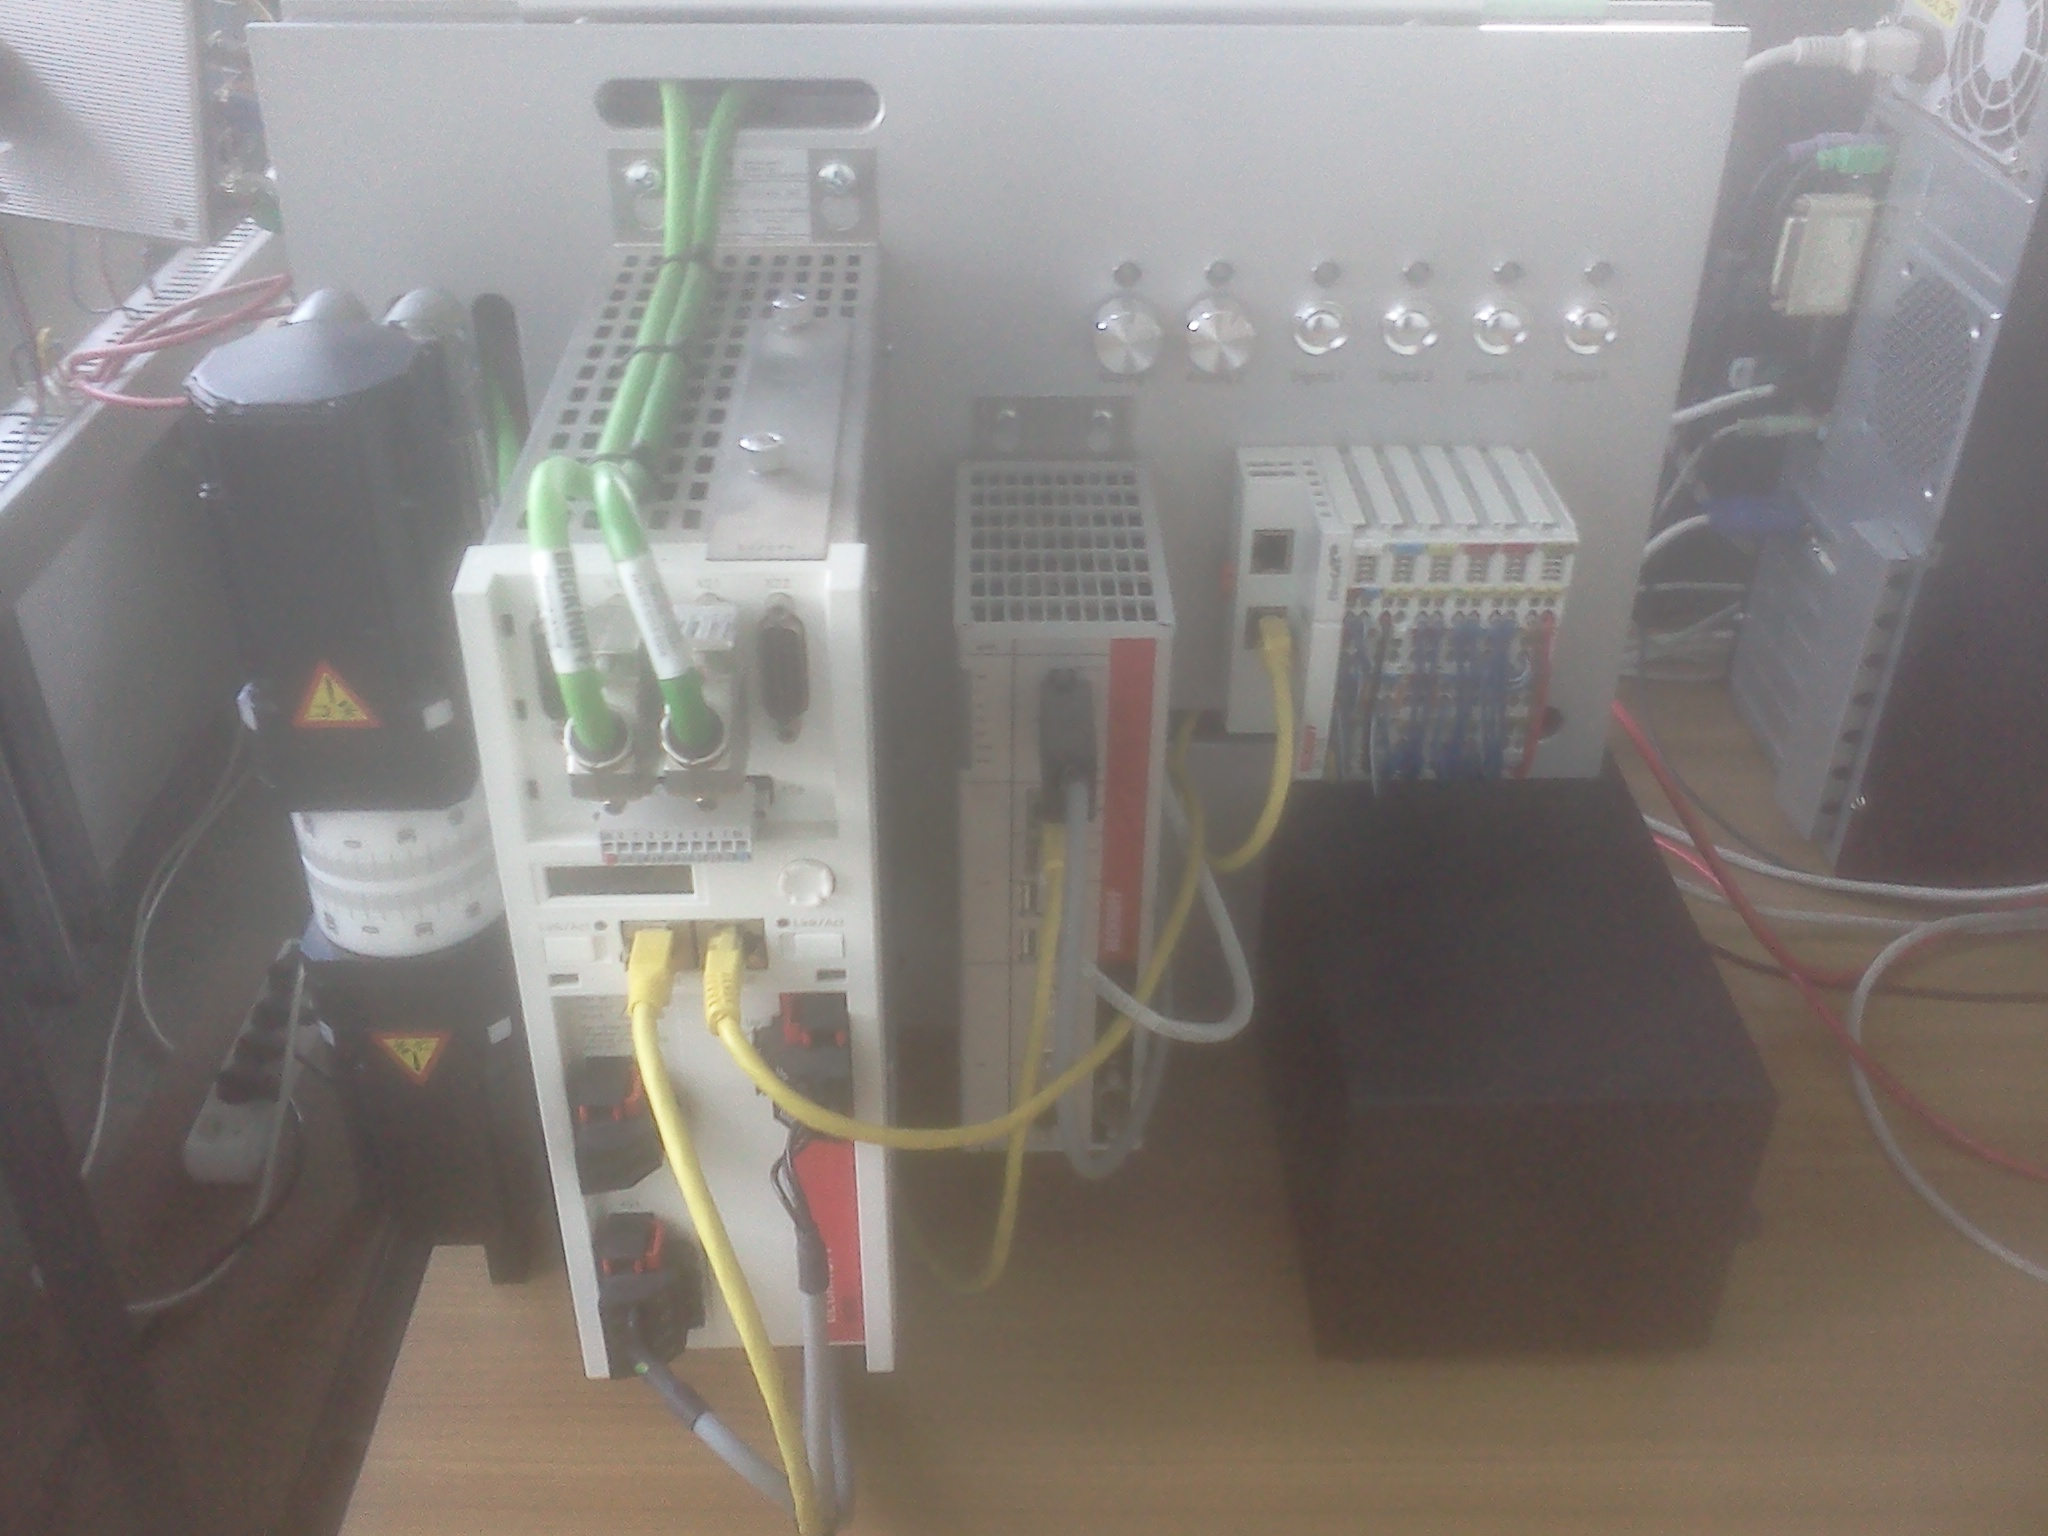
\includegraphics[height=0.85\textheight]{images/typ1.jpg}
\end{figure}
\end{frame}

\begin{frame}
\frametitle{Stanowisko typ 1}
\begin{enumerate}
    \item 2 silniki AM3021-0C00-0000
    \item Wyspa EK1100 z zestawem modułów IO
    \item Napęd serwomechnizmów AX5203(2 osiowy napęd)
    \item Komputer przemysłowy C6925
    \item Zasilacz
\end{enumerate}
\end{frame}

\begin{frame}
\frametitle{Stanowisko typ 2}
\begin{figure}[!htb]	
\centering 	          
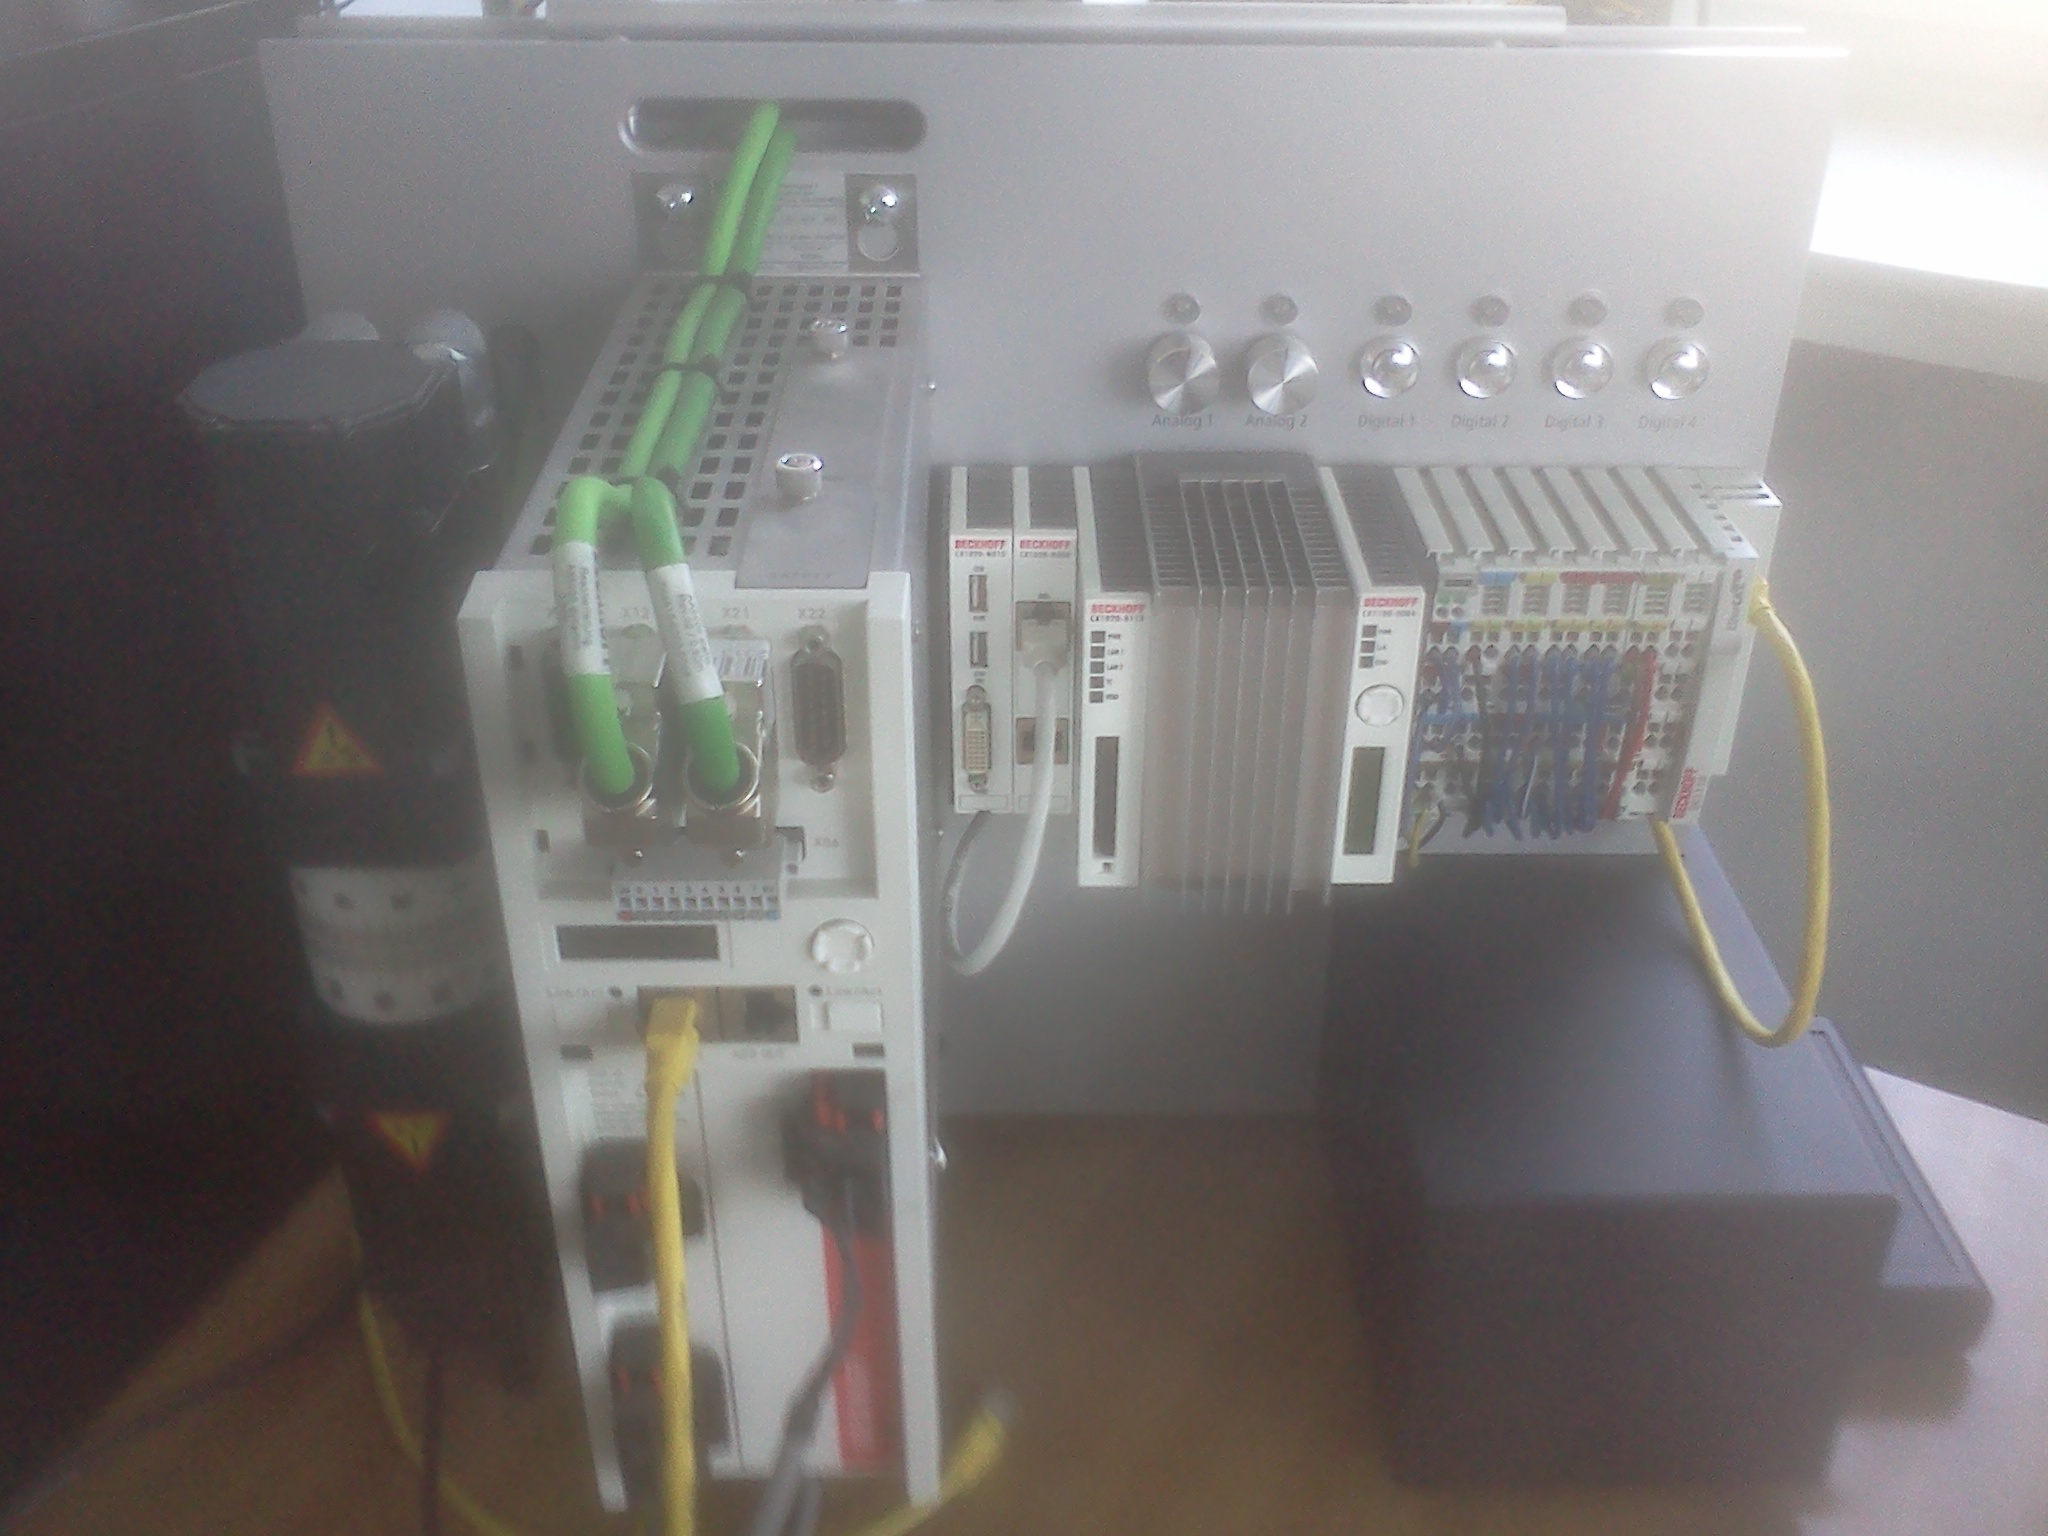
\includegraphics[height=0.85\textheight]{images/typ2.jpg}
\end{figure}
\end{frame}

\begin{frame}
\frametitle{Stanowisko typ 2}
\begin{enumerate}
    \item 2 silniki AM3021-0C00-0000
    \item Wyspa EK1100 z zestawem modułów IO
    \item Napęd serwomechnizmów AX5203(2 osiowy napęd)
    \item Modułowy komputer przemysłowy CX1020
    \item Zasilacz
\end{enumerate}
\end{frame}

\subsection{Aktualny stan pracy}
\begin{frame}
\begin{enumerate}
    \item Przejrzenie dostępnego sprzętu
    \item Zapoznawanie się z dokumentacjami i środowiskiem
\end{enumerate}
\end{frame}
\begin{frame}
\frametitle{Pytania}
Czas na pytania.
\end{frame}

\begin{frame}
\frametitle{Podsumowanie}
Dziękuję za uwagę.
\end{frame}

\end{document}
